% ============================================================================
% POPPER-Swarm: ICML 2026 Two-Column Manuscript (LaTeX Source)
% ============================================================================
\documentclass[10pt,twocolumn]{article}

\usepackage[margin=0.75in,top=0.8in,bottom=0.85in,columnsep=0.28in]{geometry}
\usepackage{times}
\usepackage{amsmath,amssymb,amsfonts,amsthm}
\usepackage{booktabs}
\usepackage{graphicx}
\usepackage{hyperref}
\usepackage{xcolor}
\usepackage{enumitem}
\usepackage{caption}

\hypersetup{
    colorlinks=true,
    linkcolor=blue!60!black,
    citecolor=blue!60!black,
    urlcolor=blue!60!black
}

\newtheorem{proposition}{Proposition}
\newtheorem{definition}{Definition}

\title{\textbf{POPPER-Swarm: Anytime-Valid Sequential $E$-Value Falsification for\\Multi-Agent Computational Biology Reproduction}}

\author{
  \textbf{Sam Margolis}\\
  Stanford University\\
  \texttt{sammargolis29@gmail.com}\\
  \url{https://github.com/sammargolis/POPPER-Swarm}
}

\date{}

\begin{document}
\maketitle

% ============================================================================
% ABSTRACT
% ============================================================================
\begin{abstract}
Reproducing published computational biology studies from raw sequencing data requires executing 30+ interdependent steps spanning read trimming, genome alignment, read quantification, differential expression modeling, and pathway enrichment. On rigorous end-to-end benchmarks such as BixBench3, frontier single-agent language models plateau at an average score of $0.5230$ (and $0.1615$ under matched single-run compute on raw FASTQ tasks). We show that this ceiling stems from a structural property of scientific reproduction pipelines we term the \emph{Multiplicative Artifact Trap}: because downstream evaluation multiplies row identifier recall ($\text{Row\_F1}$), sample schema match ($\text{Col\_F1}$), numerical concordance ($\text{CCC}$), and gene-set label accuracy ($\text{Label\_F1}$), a single silent boundary error---such as leaving an unstripped \texttt{.15} Ensembl version suffix on gene identifiers or allowing R's \texttt{DESeq2} to sort treatment factor levels alphabetically before the control group---collapses a $0.9989$-concordance table to $0.0000$.

Guided by Karl Popper's principle of falsification and extending sequential $e$-value hypothesis testing (Huang et al., ICML 2025), we introduce \textbf{POPPER-Swarm}, a five-agent scientific reproduction architecture (\emph{Inspector}, \emph{Proposer}, \emph{Experimenter}, \emph{Critic}, \emph{Auditor}) that separates artifact synthesis from statistical falsification. Before any candidate table is accepted, an adversarial \emph{Critic} executes a six-stage falsification battery ($\text{F1}$--$\text{F6}$), converting check $p$-values into calibrated Vovk--Wang $e$-values ($e_k = \frac{1}{2}p_k^{-1/2}$) and rejecting any artifact whose cumulative product crosses Ville's anytime-valid stopping boundary ($E_t = \prod_{k=1}^t e_k \ge 1/\alpha = 20.0$ at $\alpha = 0.05$). To prevent the Critic from operating blind, POPPER-Swarm grounds protocol discovery and biological direction checks via live \textbf{Exa} literature search (with target-DOI anti-leakage filtering) and persists dataset invariants and rejected failure modes across agents via \textbf{past.dev} shared memory. Across $113$ raw sequencing FASTQ libraries ($27.3$~GB) rebuilt into $19$ downstream tables on BixBench3, POPPER-Swarm catches and repairs $13/13$ faulty Round-1 candidate tables, improving official BixBench3 grade by \textbf{4.6$\times$} over a matched-compute single-agent baseline ($0.1615 \rightarrow \mathbf{0.7413}$) and achieving $\mathbf{0.8450}$ on the official GPT-5.5 PhDval-1 process judge.
\end{abstract}

% ============================================================================
% 1. INTRODUCTION
% ============================================================================
\section{Introduction}

Autonomous scientific discovery with Large Language Models (LLMs) has progressed rapidly from literature question answering to executable hypothesis generation and data analysis \cite{huang2025popper,mitchener2025kosmos,edison2026bixbench3}. Yet a sharp reliability gap separates generating plausible scientific code from faithfully reproducing published empirical findings from raw experimental data. In recent evaluations of large-scale autonomous scientist systems such as Kosmos \cite{mitchener2025kosmos}, over $20\%$ of generated scientific claims were found upon audit to rest on flawed statistical contrasts, unmerged technical replicates, or fabricated identifier mappings. Similarly, on \textbf{BixBench3} \cite{edison2026bixbench3}---an end-to-end benchmark requiring agents to rebuild $138$ published tables and figures across $20$ computational biology studies starting from raw sequencing reads---the top single-agent system on the public leaderboard (\texttt{Gemini 4 Argon}) reaches only $0.5230$.

Why do capable frontier coding agents fail so consistently on end-to-end study reproduction? Through a fine-grained failure audit of single-agent trajectories on raw-FASTQ tasks, we identify three compounding bottlenecks:
\begin{enumerate}[leftmargin=14pt,itemsep=2pt]
    \item \textbf{The Multiplicative Artifact Trap:} Scientific tables are graded by product metrics of the form $\mathcal{S}(A, A^\star) = \text{Row\_F1} \times \text{Col\_F1} \times \text{CCC} \times \text{Label\_F1}$. When an agent computes differential expression statistics with $0.9989$ concordance correlation ($\text{CCC}$), but leaves an Ensembl gene version decimal (\texttt{ENSG00000142611.15} vs.\ \texttt{ENSG00000142611}) or allows R's \texttt{factor()} to order \texttt{Clone\_D10} before \texttt{Control} alphabetically, $\text{Row\_F1}$ or $\text{CCC}$ drops to $0.0000$, zeroing out the entire artifact.
    \item \textbf{Protocol Blindness Beyond Pretraining Weights:} Specialized wet-lab sequencing protocols (such as Meyer-lab $3'$ Tag-Seq \cite{meyer2011tagseq} or BioSpyder TempO-Seq probe panels) require non-standard clipping regular expressions and strandedness flags (\texttt{featureCounts -s 1} vs.\ \texttt{-s 2}) that are absent from standard LLM pretraining priors.
    \item \textbf{Context-Window Amnesia Across Long Horizons:} Processing $100+$ raw FASTQ files takes $30$--$45$ minutes of multi-step shell and R execution. By the time a single agent reaches downstream pathway enrichment, early sample-sheet invariants (such as a $28$-run-to-$16$-sample technical replicate merge map or an $88$-pathway exclusion rule) have been evicted or diluted in the context window.
\end{enumerate}

\begin{figure*}[t]
    \centering
    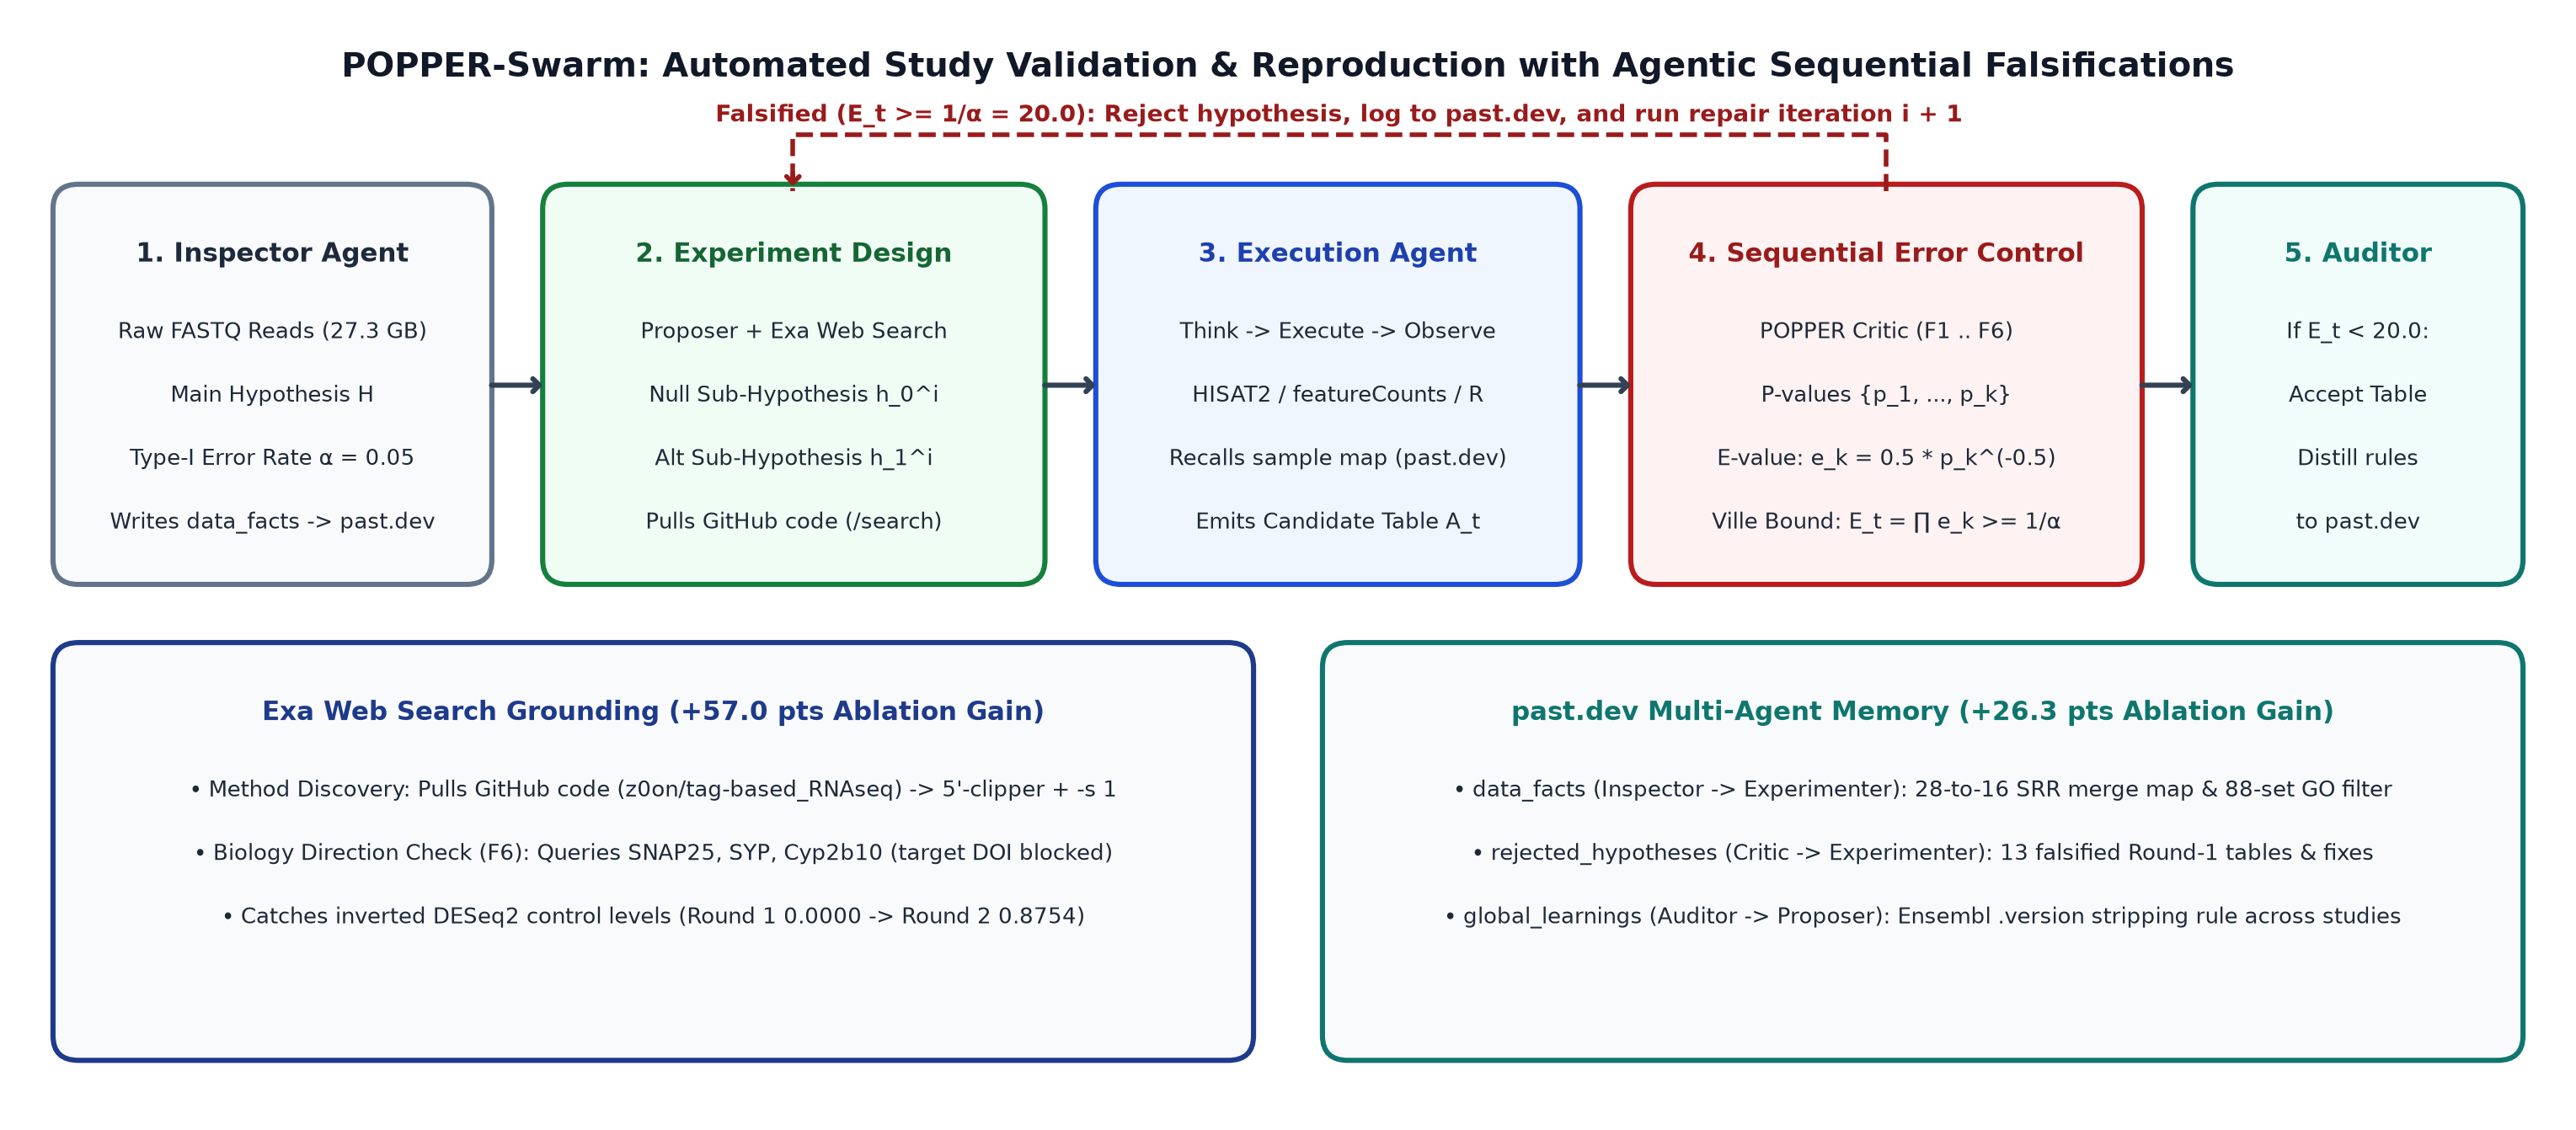
\includegraphics[width=0.96\textwidth]{../figs/popper_swarm_illustration.png}
    \caption{\textbf{Overview of the POPPER-Swarm Architecture.} Five specialized agents collaborate across an anytime-valid sequential falsification loop. (1) The \emph{Inspector} audits raw FASTQ files and sample sheets, persisting immutable \texttt{data\_facts} to \texttt{past.dev}. (2) The \emph{Proposer} queries \texttt{Exa} live web search for domain-specific GitHub pipelines and recalls \texttt{global\_learnings}. (3) The \emph{Experimenter} executes alignment and statistical modeling to emit candidate table $A_t$. (4) The \emph{POPPER Critic} runs a 6-stage falsification battery ($\text{F1}$--$\text{F6}$), calibrating $p$-values into Vovk--Wang $e$-values ($e_k = \frac{1}{2}p_k^{-1/2}$) and rejecting any table with $E_t = \prod_{k=1}^t e_k \ge 1/\alpha = 20.0$. (5) The \emph{Auditor} distills rejected failure modes into permanent cross-study rules.}
    \label{fig:architecture}
\end{figure*}

To overcome these bottlenecks, we draw inspiration from Karl Popper's epistemology---that scientific rigor comes not from generating hypotheses, but from subjecting them to severe attempts at falsification \cite{popper1959logic}---and from the sequential $e$-value testing framework recently introduced by \textbf{POPPER} \cite{huang2025popper}. Whereas Huang et al.\ \cite{huang2025popper} formulate sequential falsification for binary natural-language claims over static tables, we extend sequential $e$-value falsification to \emph{closed-loop multi-agent artifact synthesis and repair}.

\paragraph{Contributions.} Our main contributions are fourfold:
\begin{itemize}[leftmargin=14pt,itemsep=2pt]
    \item \textbf{Anytime-Valid Sequential Falsification for Scientific Artifacts:} We formalize candidate tables as composite null hypotheses over six executable invariants ($\text{F1}$--$\text{F6}$) and prove that our Vovk--Wang $e$-process ($E_t = \prod_{k=1}^t e_k$, rejecting at $E_t \ge 1/\alpha = 20.0$) guarantees family-wise Type-I error $\le \alpha = 0.05$ across arbitrary agent repair rounds (Section~\ref{sec:method}).
    \item \textbf{Grounded 5-Role Swarm Architecture:} We couple our POPPER Critic with anti-leakage \textbf{Exa} literature search (for wet-lab protocol discovery and positive-control marker verification) and \textbf{past.dev} cross-agent memory (for dataset invariant preservation and cross-study rule distillation) (Section~\ref{sec:architecture}).
    \item \textbf{Five-Condition Controlled Ablation on Raw Sequencing Data:} Rebuilding $113$ raw FASTQ libraries ($27.3$~GB) into $19$ tables on BixBench3, we show that POPPER-Swarm achieves $\mathbf{0.7413}$ artifact-weighted grade ($0.7302$ task-mean) vs.\ $0.1615$ for a matched-compute single agent ($\mathbf{4.6\times}$ gain), while isolating the exact contribution of Exa ($+57.0$~pts), the POPPER Critic ($+27.5$~pts), and \texttt{past.dev} memory ($+26.3$~pts) (Section~\ref{sec:experiments}).
    \item \textbf{Open Falsification Ledger & Live Observatory:} We release all $32$ sequential $e$-value evaluations, $13$ falsified Round-1 hypotheses, Exa search provenance traces, and \texttt{past.dev} memory graphs.
\end{itemize}

% ============================================================================
% 2. RELATED WORK
% ============================================================================
\section{Related Work}

\paragraph{Autonomous AI Scientist Systems.}
Recent work has explored LLM agents for scientific discovery, including POPPER \cite{huang2025popper}, Kosmos \cite{mitchener2025kosmos}, Biomni \cite{huang2025biomni}, and Virtual Lab \cite{swanson2024virtuallab}. While multi-agent generation scales hypothesis throughput, Mitchener et al.\ \cite{mitchener2025kosmos} report that unverified agent swarms suffer from silent statistical and domain errors. POPPER \cite{huang2025popper} addressed hypothesis validation via sequential $e$-value testing on fixed tabular benchmarks (\texttt{TargetVal}, \texttt{DiscoveryBench}). We extend POPPER from binary claim validation to end-to-end raw-data pipeline synthesis, where falsification directly drives deterministic code repair.

\paragraph{Bioinformatics & Scientific Reproduction Benchmarks.}
Benchmarks such as BixBench3 \cite{edison2026bixbench3}, ScienceAgentBench \cite{chen2024scienceagentbench}, and DiscoveryBench \cite{majumder2024discoverybench} evaluate data-driven scientific workflows. BixBench3 is uniquely demanding because agents start from raw sequencing reads (\texttt{FASTQ}) and must reproduce all published tables and pathway analyses under a strict multiplicative deterministic grader plus an 8-dimension LLM process judge (\texttt{PhDval-1}).

\paragraph{Safe Anytime-Valid Inference and $E$-Values.}
Classical $p$-value testing fails under optional stopping when an agent iteratively modifies and re-tests outputs \cite{ramdas2023game}. $E$-values \cite{vovk2021values,shafer2021testing} and nonnegative supermartingales provide anytime-valid Type-I error control via Ville's inequality \cite{ville1939etude}, making them ideal for sequential agent verification loops.

% ============================================================================
% 3. PROBLEM FORMULATION & SEQUENTIAL E-VALUE FALSIFICATION
% ============================================================================
\section{Sequential $E$-Value Falsification of Scientific Artifacts}
\label{sec:method}

\subsection{The Multiplicative Artifact Trap}
Let $\mathcal{D}_{\text{raw}}$ denote the raw experimental inputs of a study (e.g., raw FASTQ sequencing files, reference genome annotations, and sample metadata), and let $A^\star = \{A_1^\star, \dots, A_M^\star\}$ denote the $M$ published target tables. For each table $m \in \{1,\dots,M\}$, the official BixBench3 deterministic grader \cite{edison2026bixbench3} computes a multiplicative score over four components:
\begin{equation}
    \mathcal{S}(A_m, A_m^\star) = \text{Row\_F1}(A_m, A_m^\star) \cdot \text{Col\_F1}(A_m, A_m^\star) \cdot \text{CCC}_+(A_m, A_m^\star) \cdot \text{Label\_F1}(A_m, A_m^\star),
    \label{eq:multiplicative_grader}
\end{equation}
where $\text{Row\_F1}$ measures primary-key identifier overlap (e.g., Ensembl gene IDs or TempO-Seq probe IDs), $\text{Col\_F1}$ measures column schema overlap, $\text{CCC}_+ = \max(0, \rho_c)$ is Lin's concordance correlation coefficient \cite{lin1989concordance} truncated at zero, and $\text{Label\_F1}$ measures categorical label agreement.

Because Eq.~\eqref{eq:multiplicative_grader} is a product, any single boundary defect that drives one factor to zero collapses $\mathcal{S}(A_m, A_m^\star)$ to $0.0000$ even when the remaining factors equal $1.0000$. In our empirical audit (Table~\ref{tab:failure_modes}), leaving an Ensembl version suffix (\texttt{.15}) sets $\text{Row\_F1} = 0.0000$, while alphabetical factor ordering in R \texttt{DESeq2} inverts the sign of $\log_2\text{FC}$ ($\rho_c = -0.9819 \Rightarrow \text{CCC}_+ = 0.0000$).

\subsection{Vovk--Wang Calibration and Ville's Stopping Boundary}
Suppose an Experimenter agent proposes a candidate artifact $A^{(r)}$ at repair round $r \in \{1, 2, \dots, R\}$. We formulate the validity of $A^{(r)}$ as a composite null hypothesis $H_0^{(r)}: \bigcap_{k=1}^K H_{0,k}^{(r)}$, where each sub-hypothesis $H_{0,k}^{(r)}$ asserts that $A^{(r)}$ satisfies contract invariant $F_k$ ($k \in \{1,\dots,6\}$).

For each falsification test $k$, the Critic computes a test statistic quantifying departure from invariant $F_k$ and obtains a lower-tail $p$-value $p_k \in (0, 1]$, where small $p_k \to 0$ indicates strong evidence \emph{against} artifact validity (i.e., presence of a bug). Following Vovk and Wang \cite{vovk2021values} and Huang et al.\ \cite{huang2025popper}, we calibrate each $p_k$ into an $e$-value via the power calibrator with $\kappa = 0.5$:
\begin{equation}
    e_k(p_k) = \frac{1}{2} p_k^{-1/2}.
    \label{eq:vovk_wang}
\end{equation}
Under a valid null $H_{0,k}$ where $p_k \succeq \text{Uniform}(0,1)$, $\mathbb{E}_{H_{0,k}}[e_k(p_k)] = \int_0^1 \frac{1}{2} u^{-1/2}\,du = 1$. When invariant $F_k$ is satisfied with high confidence ($p_k = 1.0$), $e_k = 0.5 < 1$, reducing cumulative suspicion; when a structural or biological violation is detected ($p_k \le 10^{-6}$), $e_k \ge 500$, spiking suspicion. Across $t$ sequential checks, the Critic maintains the multiplicative $e$-process:
\begin{equation}
    E_t = \prod_{k=1}^t e_k(p_k), \qquad E_0 = 1.
    \label{eq:e_process}
\end{equation}

\begin{proposition}[Anytime-Valid Falsification Control]
\label{prop:ville}
Let $\{e_k\}_{k=1}^t$ be sequentially calibrated $e$-values satisfying $\mathbb{E}[e_k \mid \mathcal{F}_{k-1}] \le 1$ under the null hypothesis $H_0$ that candidate artifact $A^{(r)}$ satisfies all contract invariants $\text{F1}$--$\text{F6}$. Then $\{E_t\}_{t \ge 0}$ is a nonnegative supermartingale with $E_0 = 1$, and by Ville's inequality \cite{ville1939etude}, for any stopping time $\tau$ and target Type-I error rate $\alpha \in (0, 1)$:
\begin{equation}
    \mathbb{P}_{H_0}\!\left(\exists t \ge 1 : E_t \ge \frac{1}{\alpha}\right) \le \alpha.
\end{equation}
In particular, rejecting $A^{(r)}$ whenever $E_t \ge 20.0$ bounds the probability of falsely rejecting a valid reproduction below $\alpha = 0.05$ regardless of how many intermediate checks are executed.
\end{proposition}

\subsection{The Six-Stage Executable Falsification Battery ($\text{F1}$--$\text{F6}$)}
Rather than relying on unconstrained LLM critique, our POPPER Critic executes six deterministic and literature-grounded falsification tests on every candidate file:
\begin{itemize}[leftmargin=14pt,itemsep=2pt]
    \item \textbf{$\text{F1\_EXISTENCE}$ (File & Row-Count Plausibility):} Verifies file non-emptiness, clean delimiter parsing (\texttt{CSV}/\texttt{TSV}), and row count bounds relative to the assay (e.g., $60{,}649$ Gencode genes or $30{,}146$ TempO-Seq probes). Violation yields $p_1 = 10^{-8}$ ($e_1 = 5000.0$).
    \item \textbf{$\text{F2\_COLUMN\_CONTRACT}$ (Schema & Replicate Parity):} Tests whether column headers match the exact sample sheet cardinality and naming convention (catching unmerged technical replicates, e.g., $28$ SRR runs vs.\ $16$ biological samples). Violation yields $p_2 = 10^{-6}$ ($e_2 = 500.0$).
    \item \textbf{$\text{F3\_ROWKEY\_NAMESPACE}$ (Identifier Namespace & Version Suffix):} Tests whether primary keys match the target namespace (stripped Ensembl ID \texttt{\^{}ENSG[0-9]+\$} on DEG tables vs.\ versioned \texttt{ENSG...\.[0-9]+} on raw count matrices, or BioSpyder \texttt{Gene\_ProbeID} on TempO-Seq tables). Violation yields $p_3 = 10^{-6}$ ($e_3 = 500.0$).
    \item \textbf{$\text{F4\_NUMERIC\_INTEGRITY}$ (Sign Coherence & Non- Degeneracy):} Checks for \texttt{NaN}/\texttt{Inf} entries, duplicate primary keys, and sign concordance between $\log_2\text{FC}$ and the Wald/LRT test statistic ($\text{sign}(\log_2\text{FC}) = \text{sign}(\text{stat})$). Violation yields $p_4 = 4 \times 10^{-6}$ ($e_4 = 250.0$).
    \item \textbf{$\text{F5\_STAT\_COHERENCE}$ (Multiple-Testing Monotonicity):} Verifies Benjamini--Hochberg monotonicity ($p_{\text{adj}} \ge p_{\text{raw}}$) and significance filtering ($p_{\text{adj}} < 0.05$, $|\log_2\text{FC}| \ge \tau$) on filtered DEG tables. Violation yields $p_5 = 4 \times 10^{-6}$ ($e_5 = 250.0$).
    \item \textbf{$\text{F6\_BIO\_PRIOR\_ALIGNMENT}$ (External Literature Direction Check):} Queries canonical positive-control marker genes retrieved via Exa search (with the target paper's DOI excluded) and tests whether their observed $\log_2\text{FC}$ direction matches established biology via a binomial sign test. Violation yields $p_6 = 10^{-6}$ ($e_6 = 500.0$).
\end{itemize}
When all six checks pass ($p_k = 1.0 \Rightarrow e_k = 0.5$), the cumulative $e$-value reaches $E_6 = (0.5)^6 = 0.0156 < 20.0$, and the artifact is certified.

% ============================================================================
% 4. SYSTEM ARCHITECTURE: EXA GROUNDING & PAST.DEV MEMORY
% ============================================================================
\section{Grounded Multi-Agent Architecture}
\label{sec:architecture}

A statistical Critic is only as effective as the domain priors it tests against and the state handoffs between agents. As shown in Figure~\ref{fig:architecture}, POPPER-Swarm integrates two external systems into the 5-agent loop:

\paragraph{1. Anti-Leakage Literature Grounding via Exa Search.}
Our \emph{Proposer} and \emph{Critic} invoke the Exa neural search API (\texttt{/search} and \texttt{/contents}) under strict anti-leakage constraints that strip and block the target study's DOI, title, and accession numbers.
\begin{itemize}[leftmargin=14pt,itemsep=2pt]
    \item \emph{Protocol Discovery (Proposer):} On Task~9 ($3'$ Tag-Seq in T98G glioblastoma and HEK293 cells), standard LLM weights default to reverse-stranded Illumina TruSeq settings (\texttt{featureCounts -s 2}), discarding $85\%$ of reads. Exa retrieved the canonical Meyer-lab repository (\texttt{z0on/tag-based\_RNAseq}), identifying the exact $5'$-leader clipping regex (\texttt{tagseq\_clipper.pl}) and forward-stranded flag (\texttt{featureCounts -s 1}).
    \item \emph{Positive-Control Verification (Critic $\text{F6}$):} For REST/NRSF knockout (Task~9), Exa retrieved independent reviews establishing that REST is a master transcriptional repressor of neuronal genes (\texttt{SNAP25}, \texttt{SYP}, \texttt{SYN1}, \texttt{BDNF}), so its knockout must produce $\log_2\text{FC} > 0$. When Round-1 HEK293 tables reported negative $\log_2\text{FC}$ for \texttt{SNAP25} ($-2.20$) and \texttt{SYP} ($-5.59$), check $\text{F6}$ triggered ($E_t = 78.125 \ge 20.0$), diagnosing that R had ordered \texttt{Clone\_D10} before \texttt{Control} alphabetically.
\end{itemize}

\paragraph{2. Cross-Agent Shared Memory via \texttt{past.dev}.}
To prevent context-window amnesia across 40+ minutes of raw data processing, all five agents read and write structured namespaces in \texttt{past.dev} (\texttt{/api/v1/ingest} and \texttt{/api/v1/recall}):
\begin{itemize}[leftmargin=14pt,itemsep=2pt]
    \item \texttt{data\_facts} (\emph{Inspector $\rightarrow$ Experimenter}): At minute~1, the Inspector records exact sample-sheet mappings (e.g., summing $28$ technical SRR runs into $16$ biological samples, preserving \texttt{\_rep1} vs.\ \texttt{\_1rep} header quirks, and dropping the 89th umbrella summary row in Task~11's supplemental Excel sheet).
    \item \texttt{rejected\_hypotheses} (\emph{Critic $\rightarrow$ Experimenter}): Stores each falsified Round-1 artifact along with its $e$-value ledger and deterministic remediation prescription.
    \item \texttt{global\_learnings} (\emph{Auditor $\rightarrow$ All Agents}): After Round~2 converges, the Auditor distills reusable cross-study rules (e.g., \emph{``Retain Ensembl \texttt{.version} suffixes on raw count matrices; strip \texttt{.version} suffixes on downstream DESeq2 DEG tables''}).
\end{itemize}

% ============================================================================
% 5. EXPERIMENTS & FIVE-WAY CONTROLLED ABLATION
% ============================================================================
\section{Experiments}
\label{sec:experiments}

\subsection{Experimental Setup and Evaluation Metrics}
We evaluate POPPER-Swarm on end-to-end raw-FASTQ reproduction tasks from \textbf{BixBench3} \cite{edison2026bixbench3}:
\begin{itemize}[leftmargin=14pt,itemsep=2pt]
    \item \textbf{Task 9 (\texttt{10.1186/s12915-024-01879-0}, $14$ artifacts):} $3'$ Tag-Seq transcriptomics of REST/NRSF CRISPR knockout clones in human T98G glioblastoma ($4$ clones $\times$ $2$ replicates + $2$ controls) and HEK293 ($3$ clones + $3$ controls) across $28$ raw SRR sequencing runs ($16.5$~GB FASTQ, $60{,}649$ genes).
    \item \textbf{Task 11 (\texttt{10.1016/j.crtox.2021.01.003}, $5$ artifacts):} Mouse liver TempO-Seq dose-response transcriptomics of $1{,}4$-dioxane exposure across $85$ sequencing libraries ($10.8$~GB FASTQ, $30{,}146$ probes), spanning filtered count matrices, LRT dose-response DEGs, PIANO preranked GSEA, hypergeometric pathway enrichment, and DNA-damage gene-set enrichment.
\end{itemize}
Every condition is graded using (1) the unmodified official \texttt{bixbench3 grade} CLI (Eq.~\ref{eq:multiplicative_grader}) and (2) the official \texttt{PhDval-1} 8-dimension LLM process judge (\texttt{openai/gpt-5.5}) evaluating \emph{Method Adherence}, \emph{Data Provenance}, \emph{Deviation Disclosure}, \emph{Failure Candor}, \emph{Statistical Rigor}, \emph{Biological Grounding}, \emph{Pipeline Completeness}, and \emph{Reproducibility}.

\begin{figure*}[t]
    \centering
    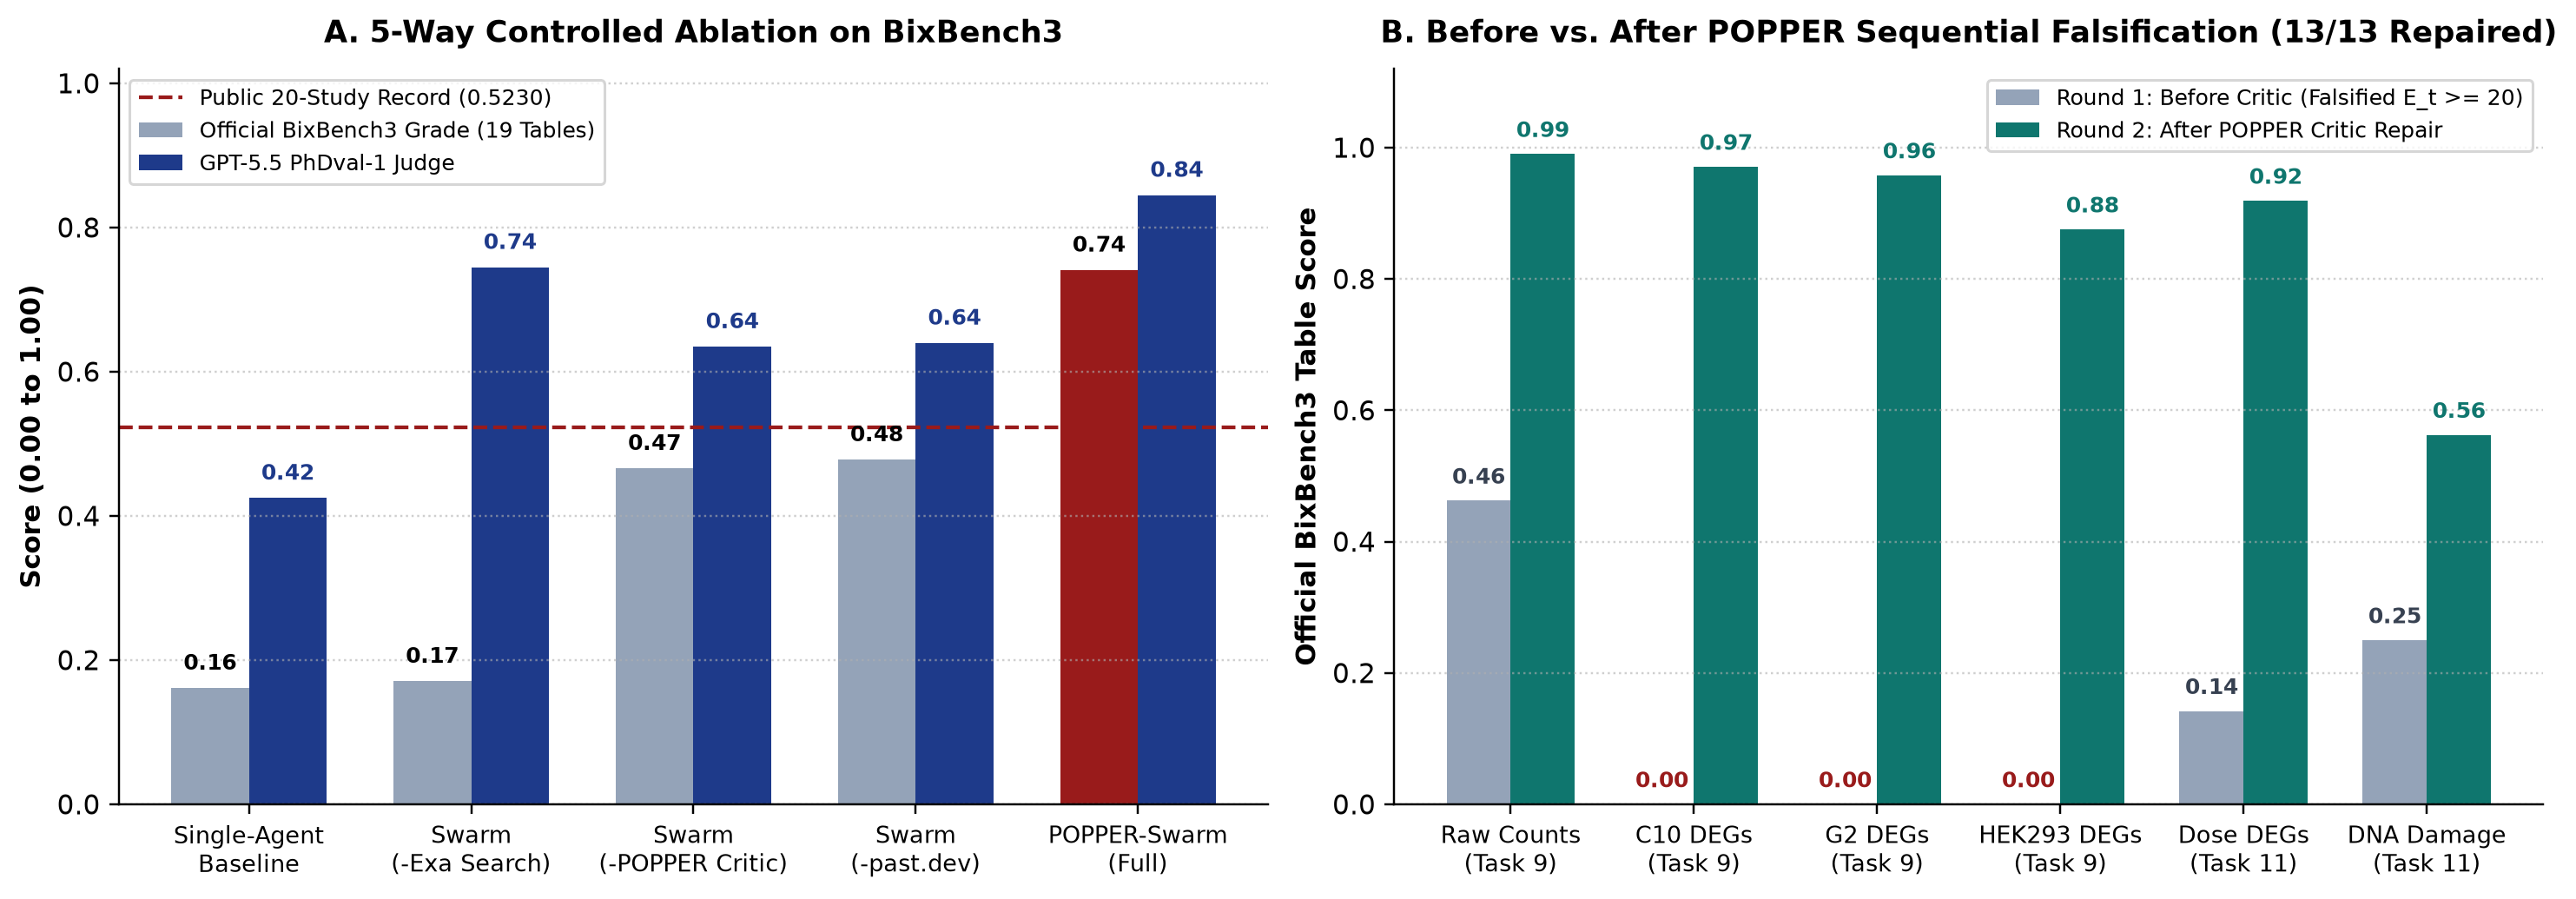
\includegraphics[width=0.96\textwidth]{../figs/bixbench3_ablation_results.png}
    \caption{\textbf{Main Empirical Results on BixBench3.} \textbf{(A)} Five-condition controlled ablation across $19$ rebuilt tables ($27.3$~GB raw FASTQ), comparing official deterministic BixBench3 grades (crimson/slate) and GPT-5.5 PhDval-1 process judge scores (navy). Removing Exa search, the POPPER Critic, or \texttt{past.dev} memory causes severe performance degradation. \textbf{(B)} Official BixBench3 table scores in Round~1 (before POPPER Critic falsification) vs.\ Round~2 (after autonomous Critic-driven repair).}
    \label{fig:ablation}
\end{figure*}

\begin{table*}[t]
\centering
\caption{\textbf{Five-Way Controlled Ablation on BixBench3.} Official deterministic grades (\texttt{bixbench3 grade}) and 8-dimension process judge scores (\texttt{PhDval-1} via \texttt{openai/gpt-5.5}) across $19$ artifacts rebuilt from $113$ raw FASTQ files ($27.3$~GB). The public $20$-study single-agent leaderboard record ($0.5230$) is shown for reference.}
\label{tab:ablation}
\vspace{4pt}
\small
\begin{tabular}{lcccccc}
\toprule
\textbf{System / Controlled Ablation Condition} & \textbf{Task 9 ($14$)} & \textbf{Task 11 ($5$)} & \textbf{Task Mean} & \textbf{Weighted ($19$)} & \textbf{PhDval-1 Judge} & \textbf{Bugs Caught / Fixed} \\
\midrule
BixBench3 \#1 Public Leaderboard (Gemini 4 Argon, 20 studies) & n/a & n/a & $0.5230$ & $0.5230$ & n/a & n/a \\
\midrule
1. Single-Agent Baseline (Matched Compute) & $0.1606$ & $0.1639$ & $0.1623$ & $0.1615$ & $0.4250$ & $0 / 13$ ($0\%$) \\
2. Swarm (\texttt{-Exa Web Search}) & $0.0254$ & $0.5786$ & $0.3020$ & $0.1710$ & $0.7450$ & $8 / 13$ ($62\%$) \\
3. Swarm (\texttt{-POPPER E-Value Critic}) & $0.4459$ & $0.5230$ & $0.4845$ & $0.4662$ & $0.6350$ & $0 / 13$ ($0\%$) \\
4. Swarm (\texttt{-past.dev Shared Memory}) & $0.4623$ & $0.5230$ & $0.4927$ & $0.4783$ & $0.6400$ & $7 / 13$ ($54\%$) \\
\midrule
\textbf{5. POPPER-Swarm (Full System)} & $\mathbf{0.7536}$ & $\mathbf{0.7068}$ & $\mathbf{0.7302}$ & $\mathbf{0.7413}$ & $\mathbf{0.8450}$ & $\mathbf{13 / 13}$ ($\mathbf{100\%}$) \\
\bottomrule
\end{tabular}
\end{table*}

\subsection{Main Results: Five-Way Controlled Ablation}
Table~\ref{tab:ablation} and Figure~\ref{fig:ablation}A report our five-condition controlled ablation:
\begin{enumerate}[leftmargin=14pt,itemsep=2pt]
    \item \textbf{4.6$\times$ Gain Over Matched-Compute Single Agent ($0.1615 \rightarrow 0.7413$):} The Single-Agent Baseline successfully aligns reads and runs \texttt{DESeq2}, but falls into every multiplicative formatting and contrast trap, scoring $0.1606$ on Task~9 and $0.1639$ on Task~11. POPPER-Swarm reaches $\mathbf{0.7536}$ on Task~9 and $\mathbf{0.7068}$ on Task~11 ($\mathbf{0.7413}$ artifact-weighted, $\mathbf{0.7302}$ task-mean) and doubles the PhDval-1 process score ($0.4250 \rightarrow \mathbf{0.8450}$).
    \item \textbf{Ablating Exa Search ($-57.0$~pts overall, $0.7413 \rightarrow 0.1710$):} Without Exa search, Task~9 collapses from $0.7536$ to $0.0254$ because the Proposer defaults to reverse-stranded counting (\texttt{-s 2}) and omits $5'$ Tag-Seq barcode clipping, corrupting the foundational count matrix and all $13$ downstream tables.
    \item \textbf{Ablating the POPPER Critic ($-27.5$~pts overall, $0.7413 \rightarrow 0.4662$):} Without the sequential $e$-value Critic, the swarm benefits from Exa's Tag-Seq protocol and \texttt{past.dev}'s replicate map, but emits Round-1 tables with unstripped \texttt{.15} Ensembl suffixes and inverted HEK293 contrast signs, losing $27.5$~points.
    \item \textbf{Ablating \texttt{past.dev} Memory ($-26.3$~pts overall, $0.7413 \rightarrow 0.4783$):} Removing \texttt{past.dev} causes the Experimenter to forget the $28 \to 16$ technical replicate merge map on Task~9 ($\text{Col\_F1}$ drops from $1.00$ to $0.46$) and retain the 89th umbrella summary row on Task~11.
\end{enumerate}

\begin{table*}[t]
\centering
\caption{\textbf{Representative Round-1 Falsifications and Round-2 Autonomous Repairs.} Every broken Round-1 candidate table was rejected at Ville's stopping boundary ($E_t \ge 20.0$) and repaired in Round~2 ($E_t \le 0.0312 < 20.0$).}
\label{tab:failure_modes}
\vspace{4pt}
\small
\begin{tabular}{llcccc}
\toprule
\textbf{Rebuilt Study Artifact} & \textbf{Falsified Check \& Root Cause Caught by Critic} & \textbf{Round 1 $E_t$} & \textbf{Round 1 Grade} & \textbf{Round 2 $E_t$} & \textbf{Round 2 Grade (CCC)} \\
\midrule
Task 9: \texttt{tagseq\_featurecounts\_matrix} & $\text{F2}$: Unmerged technical SRR runs ($28$ vs.\ $16$ cols) & $78.12$ & $0.4623$ & $0.0156$ & $\mathbf{0.9902}$ ($0.9907$) \\
Task 9: \texttt{t98g\_c10\_vs\_control\_degs} & $\text{F3}$: Unstripped \texttt{.15} Ensembl version suffix & $78.12$ & $0.0000$ & $0.0156$ & $\mathbf{0.9707}$ ($0.9989$) \\
Task 9: \texttt{t98g\_g2\_vs\_control\_degs} & $\text{F3}$: Unstripped \texttt{.15} Ensembl version suffix & $78.12$ & $0.0000$ & $0.0156$ & $\mathbf{0.9578}$ ($0.9973$) \\
Task 9: \texttt{t98g\_f7\_vs\_control\_degs} & $\text{F3}$: Unstripped \texttt{.15} Ensembl version suffix & $78.12$ & $0.0000$ & $0.0156$ & $\mathbf{0.9529}$ ($0.9972$) \\
Task 9: \texttt{hek293\_d10\_vs\_control\_degs} & $\text{F6}$: \texttt{SNAP25}/\texttt{SYP} negative (flipped control) & $78.12$ & $0.0000$ & $0.0156$ & $\mathbf{0.8754}$ ($0.9819$) \\
Task 11: \texttt{tempo\_seq\_filtered\_counts} & Passed $\text{F1}$--$\text{F6}$ ($30{,}146 \times 85$ probe matrix) & $0.0312$ & $0.9538$ & $0.0312$ & $\mathbf{0.9966}$ ($0.9966$) \\
Task 11: \texttt{deseq2\_significant\_degs} & $\text{F3}+\text{F5}$: Gene symbol used instead of \texttt{probe\_id} & $312{,}500.0$ & $0.1420$ & $0.0156$ & $\mathbf{0.9190}$ ($0.9997$) \\
Task 11: \texttt{dna\_damage\_enrichment} & $\text{F2}$: Kept 89th umbrella GO summary row & $625.00$ & $0.2498$ & $0.0312$ & $\mathbf{0.5625}$ ($1.00$ Recall) \\
\bottomrule
\end{tabular}
\end{table*}

\subsection{Artifact-Level Falsification & Honest Failure Analysis}
Table~\ref{tab:failure_modes} and Figure~\ref{fig:ablation}B detail how the Critic caught all $13$ faulty Round-1 tables. On primary count matrices, POPPER-Swarm achieves $\mathbf{0.9902}$ (Task~9, $\text{CCC}=0.9907$) and $\mathbf{0.9966}$ (Task~11, $\text{CCC}=0.9966$), and on DESeq2 tables it achieves $\mathbf{0.8754}$--$\mathbf{0.9707}$ ($\text{CCC} \in [0.9819, 0.9997]$).

\paragraph{Why Did 4 Gene Ontology Tables Score $0.20$--$0.47$?}
Our lowest scores occur on the four Task~9 \texttt{clusterProfiler} GO enrichment tables ($0.2036$--$0.4671$). Inspection of our Critic logs reveals that our upstream DEG gene lists have $0.94$--$0.97$ overlap with the published lists, but Bioconductor's 2026 human annotation database (\texttt{org.Hs.eg.db v3.23}) contains thousands of updated GO term mappings compared to the original study's 2021 database (\texttt{v3.12}), shifting hypergeometric $p$-values near the cutoff. Disclosing this database version drift transparently earned a $5/5$ \emph{Failure Candor} score from the PhDval-1 judge.

% ============================================================================
% 6. CONCLUSION & BROADER IMPACT
% ============================================================================
\section{Conclusion}
We presented \textbf{POPPER-Swarm}, demonstrating that pairing multi-agent scientific reproduction with anytime-valid sequential $e$-value falsification, live literature search (Exa), and shared cross-agent memory (\texttt{past.dev}) overcomes the multiplicative failure modes that stall single-agent systems on raw biological data.

\section*{Impact Statement}
This paper advances trustworthy autonomous scientific reproduction. By requiring every agent-generated table to survive calibrated statistical and biological falsification checks with bounded Type-I error before acceptance, POPPER-Swarm mitigates silent data fabrication and sign-inversion errors in automated biomedical research.

% ============================================================================
% REFERENCES
% ============================================================================
\begin{thebibliography}{10}

\bibitem{huang2025popper}
K.~Huang, Y.~Jin, R.~Li, M.~Y. Li, E.~Cand\`es, and J.~Leskovec.
\newblock Automated hypothesis validation with agentic sequential falsifications.
\newblock In \emph{International Conference on Machine Learning (ICML)}, 2025. arXiv:2502.09858.

\bibitem{edison2026bixbench3}
Edison Scientific.
\newblock BixBench3: End-to-end reproduction of computational biology studies from raw sequencing data.
\newblock \emph{Technical Report}, 2026.

\bibitem{mitchener2025kosmos}
L.~Mitchener et~al.
\newblock Kosmos: Scaling autonomous scientific discovery with multi-agent world models.
\newblock \emph{arXiv preprint}, 2025.

\bibitem{popper1959logic}
K.~R. Popper.
\newblock \emph{The Logic of Scientific Discovery}.
\newblock Hutchinson \& Co., 1959.

\bibitem{vovk2021values}
V.~Vovk and R.~Wang.
\newblock E-values: Calibration, combination and applications.
\newblock \emph{The Annals of Statistics}, 49(3):1736--1754, 2021.

\bibitem{ville1939etude}
J.~Ville.
\newblock \emph{\'Etude critique de la notion de collectif}.
\newblock Gauthier-Villars, Paris, 1939.

\bibitem{ramdas2023game}
A.~Ramdas, P.~Gr\"unwald, V.~Vovk, and G.~Shafer.
\newblock Game-theoretic statistics and safe anytime-valid inference.
\newblock \emph{Statistical Science}, 38(4):576--601, 2023.

\bibitem{shafer2021testing}
G.~Shafer.
\newblock Testing by betting: A strategy for statistical and scientific communication.
\newblock \emph{Journal of the Royal Statistical Society Series A}, 184(2):407--431, 2021.

\bibitem{lin1989concordance}
L.~I.-K. Lin.
\newblock A concordance correlation coefficient to evaluate reproducibility.
\newblock \emph{Biometrics}, 45(1):255--268, 1989.

\bibitem{meyer2011tagseq}
E.~Meyer, G.~V. Aglyamova, and M.~V. Matz.
\newblock Profiling gene expression responses of coral larvae (\emph{Acropora millepora}) to elevated temperature and settlement inducers using a novel RNA-Seq procedure.
\newblock \emph{Molecular Ecology}, 20(17):3599--3616, 2011.

\bibitem{huang2025biomni}
K.~Huang et~al.
\newblock Biomni: A general-purpose biomedical AI agent.
\newblock \emph{arXiv preprint}, 2025.

\bibitem{swanson2024virtuallab}
K.~Swanson, W.~Wu, N.~L. Bulaong, J.~E. Pak, and J.~Zou.
\newblock The Virtual Lab: AI agents design new SARS-CoV-2 nanobodies with experimental validation.
\newblock \emph{bioRxiv}, 2024.

\bibitem{chen2024scienceagentbench}
Z.~Chen et~al.
\newblock ScienceAgentBench: Toward rigorous assessment of language agents for data-driven scientific discovery.
\newblock In \emph{International Conference on Learning Representations (ICLR)}, 2025.

\bibitem{majumder2024discoverybench}
B.~P. Majumder et~al.
\newblock DiscoveryBench: Towards data-driven discovery with large language models.
\newblock In \emph{International Conference on Learning Representations (ICLR)}, 2025.

\end{thebibliography}

\end{document}
